\documentclass{article}

\usepackage[utf8]{inputenc}

\usepackage[
    backend=biber,
    natbib=true
]{biblatex}
\addbibresource{plan.bib} %Import the bibliography file

\usepackage{hyperref}
\hypersetup{
    colorlinks=true,
}

\usepackage[pdf]{graphviz}
\usepackage{graphicx}
\usepackage{amsmath}
\usepackage{amsthm}
\usepackage{amssymb}

\usepackage[colorinlistoftodos]{todonotes}

\usepackage{parskip}
\setlength{\parskip}{10pt} 

\usepackage{tikz}
\usetikzlibrary{arrows, decorations.markings}

\usepackage{chngcntr}
\counterwithout{figure}{section}

\theoremstyle{definition}
\newtheorem*{ex}{Example}

\begin{document}

\begin{titlepage}

\centering
  
{\scshape\LARGE Master's thesis project plan\\}
  
\vspace{0.5cm}
  
{\huge\bfseries E-graphs modulo theories\\}
  
\vspace{2cm}
  
{\Large Sofia Brookie \\ \href{mailto:sofia.ma@protonmail.com}{sofia.ma@protonmail.com} \\}
  
\vspace{1.0cm}
  
{\large Supervisor: Nicholas Smallbone\\}
{\large Examiner: David Sands\\}

\vfill

\vfill
  
{\large \today\\} 

\end{titlepage}

\section{Overview}
This thesis project will develop the idea of \textit{E-graphs Modulo Theories}.

E-graphs are a data structure and algorithm for automatically discovering and proving equations that hold
between a set of first-order terms, given as input a starting set of terms and a theory (a set of identities). E-graphs have seen a lot of interest since the publication of the \textsc{Egg} library developed by Willsey et al. and their corresponding paper \cite{willsey2021egg}.

However, E-graphs struggle with the combinatorial explosion involved in directly reasoning about certain theories, such as those containing associative and commutative operators. Despite the existence of well-known techniques to reason about associative and commutative operators, standard E-graphs use the `generic' E-graph approach for everything, resulting in a potential exponential expansion in the E-graph size just to deduce basic consequences of the associative and commutative identities.

Zucker \cite{zucker2025omelets} proposes extending the notion of E-graphs to that of \textit{E-graphs Modulo Theories} (EMTs) in order to use much more efficient techniques to handle certain subtheories, and use the E-graph mechanisms only for the other identities in the theory. Beyond associativity and commutativity, Zucker also lists some other subtheories for which EMTs can make reasoning more efficient by using standard theory-specific techniques, such as the handling the theory of vector spaces with Gaussian elimination.

Our aim is to describe a means of implementing EMTs for the case of associativity and/or commutativity, and in particular describe solutions to \textit{matching modulo theories}, for which a na\"ive but potentially slow algorithm due to Zucker is known. We aim to show that more performant methods of matching can be implemented without losing the ability to match modulo theories.

\section{Problem formulation and background}
\subsection{Equational theories}
The problem E-graphs solve is reasoning about equations over a set of function symbols and constants. To make this precise, a \textbf{signature} is a set $\Sigma$ of function symbols with an arity given by a function $\alpha : \Sigma \rightarrow \mathbb{N}$. Given a set of constants $A$, a \textbf{term fragment}\footnote{I am unaware of a standard name for this notion.} $\Sigma(A)$ is a pair of an element of $f \in \Sigma$ together with a list of elements of $A$ of length $\alpha(f)$. A \textbf{term} over $A$, denoted by $\Sigma^*(A)$, is defined inductively as either a constant $a \in A$ or a term fragment over $\Sigma^*(A)$.

Given a term in $\Sigma^*(A)$, we can extend it to be over more constants $\Sigma^*(A + B)$ in the obvious way. We will often use auxiliary constants written as $x, y, z$ etc., but these should be distinguished from the notion of a variable in an identity below.

An interpretation of a signature $\Sigma$ is a \textit{carrier} set $A$ together with a function $a : \Sigma(A) \rightarrow A$ that interprets term fragments, from which the interpretation of terms in $\Sigma^*(A)$ is given by recursive application of $a$, interpreting from the leaves to the root in the natural way. We will denote this by $\textbf{fold}(a) : \Sigma*(A) \rightarrow A$.

Given a signature, there is a standard notion of first-order logic over the terms of $\Sigma*(A)$. More specifically, we will consider \textbf{theories}, which are conjunctions of identities, where an \textbf{identity} is a proposition of the form $\forall x_1. \dotsi \forall x_i. t_1 = t_2$ where $t_1$ and $t_2$ are terms over $A + \{x_1, \dotsc x_i\}$. Note that the number of quantifiers can also be 0.
A \textbf{ground instance} of an identity is an equation of the form $\sigma(t_1) = \sigma(t_2)$, where $\sigma$ is a \textbf{substitution} that maps variables in $\{x_1, \dotsc x_i\}$ to terms over $A$. We will generally use \textbf{equation} to mean any equation between terms in the \textbf{ground fragment} $\Sigma^*(A)$, while using identity to mean a universally quantified equation.

\begin{ex}
Let $\Sigma = \{f, g\}$ and $\alpha(f) = 2, \alpha(g) = 1$. If $A = \{x, y, z\}$, then $f(x, y)$, $g(z)$, and $f(y, y)$ are elements of $\Sigma(A)$. In addition, $x$, $f(f(x, y), g(x))$, and $g(g(g(z)$ are elements of $\Sigma^*(A)$.

If we have the theory $T = (\forall a b. f(a, b) = g(f(a, b))) \wedge (\forall a. g(a) = g(g(a)))$, then we can derive the ground equation $f(x, g(y)) = g(f(x, g(y))$ from $T$ by a substitution in the first identity of $\sigma(a) = x, \sigma(b) = g(y)$.
\end{ex}

\subsection{Congruence closure and E-graphs}
If we have a signature $\Sigma$ with only 0-ary function symbols, then deciding equality over
$\Sigma^*(A)$ for any theory is easy: we use the standard union-find data structure to represent subsets of equal terms, which are just sets of function symbols, and call union($f$, $g$) for any identity $f = g$ in the theory. We can view the union-find procedure as computing the reflexive, symmetric, transitive closure of the equality relation.

When we have function symbols with greater arity, we need to consider congruence: for instance, if $a = b$, then $f(a, c) = f(b, c)$. E-graphs were pioneered by Nelson and Oppen \cite{nelson1980fast}, as a method to represent a set of terms and the congruence closure of given equations.

An E-graph consists of a graph with a set of vertexes (E-classes) $e_i$, where each $e_i$ contains a multiset of function symbols. There are also auxiliary data structures: a union-find structure on the E-classes, and some tables for indexed lookup. See \citep{willsey2021egg} for a full specification. The edges are directed and labelled with an element $f$ of the target multiset together with an argument number $i \in \alpha(f)$. The following diagram gives some visual intution for E-graphs:

\begin{figure}[!ht] % suggests placing the figure here
    \centering % Centers the figure in the column
    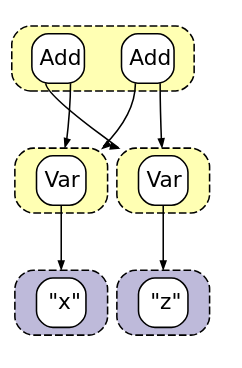
\includegraphics[width=0.3\columnwidth]{addxz}
    \caption{E-graph representing the term $x + z$ and the equation $x + z = z + x$, using egglog's visualization. Note constants are represented by Var(constant name), and also note that the top node is a multiset, containing two instances of the Add symbol}
    \label{egxzdem}
\end{figure}

There are certain well-formedness criteria for the graph to be valid, such as the fact that every symbol in a node's multiset of symbols needing as many children pointing to it as the arity of that symbol, but we will not spell this out in formal detail.

An E-graph is \textbf{canonical} if it represents the congruence closure of the given terms and equations. Not all E-graphs are canonical, but they provide a canonicalization procedure: if we have a function symbol in two different E-classes with the same argument E-class IDs, we merge those two E-classes using the union-find structure, and repeat this until we reach a fixed point.

\subsection{The saturation procedure}
Using E-graphs, one can derive consequences for a given theory over a given set of ground terms as follows:

\begin{enumerate}
	\item Insert all the starting terms into the E-graph
	\item Repeat until fixed point:
		\begin{enumerate}
		\item Match all identities against the graph, finding all ground instances of one side of the identity that exist in the graph
		\item Using the substitutions from the previous step, add the other side of the identity to the graph, suitably substituted
		\item Merge the new nodes with the nodes that they were derived from
		\item Canonicalize the graph
		\end{enumerate}
\end{enumerate}

If the fixed point is reached, we call the graph \textbf{saturated}.

Whether this procedure always terminates on a theory, and whether it deduces every consequence of that theory on the ground terms, depend on the theory in question.

\subsection{Associativity and commutativity}
Given a binary function symbol $f$, the
associativity identity is $\forall abc. f(a, f(b, c)) = f(f(a, b), c)$ and the commutativity identity is $\forall ab. f(a, b) = f(b, a)$. These identities arise in the theory of many operators (such as concatenation, multiplication, addition, union, intersection, and exclusive-OR).

While E-graphs equality saturation is designed to handle any set of identities, associativity and commutativity lead to an explosion in the size of the E-graph when it is saturated, as the number of equivalence classes of subterms of a term with $n$ occurences of an associative and/or commutative function is proportional to $\exp(n)$. Even if applying identities stops before saturation, it is likely that a large number of `useless' associativity/commutativity steps will have been taken.

We will show some examples of E-graphs handling associativity and commutativity for a function called `Add', on input terms of increasing size. We will also use the binary operator $+$ as the function symbol for `Add'. We use the online Egglog demo \cite{egglogdemo} to apply the rules and generate the resulting E-graph.
In the smallest example (Figure \ref{egxz}), using just the term $x + z$, the E-graph will run to saturation, and
give us three equivalence classes: $\{x\}$, $\{z\}$, and $\{x + z, z + x\}$.

\begin{figure}[!ht] % suggests placing the figure here
    \centering % Centers the figure in the column
    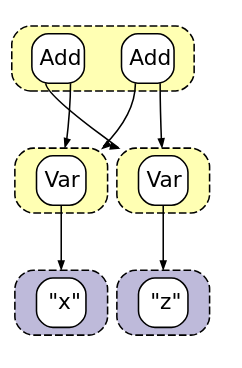
\includegraphics[width=0.3\columnwidth]{addxz}
    \caption{E-graph of the term $x + z$ after rewriting to saturation.}
    \label{egxz}
\end{figure}

Each yellow box is an equivalence class of terms that the E-graph algorithm has discovered by applying identities, and each white node inside a yellow box is the root function of one of the equivalent terms.

The process is to add the input terms to the graph. Then, we \emph{match} either the left-hand or right-hand side of an identity to the graph. In our example, we match $a + b$ to $x + y$ in the natural way. Then we add a term for the other side of the equation to the graph, and merge the resulting node with our original one to represent that they are equal. In this case, the we have $x + z$ matching the left-hand side of the identity $a + b = b + a$, so we add the term $z + x$ to the graph, and merge its equivalence class with that of $x + z$. We can then apply the identity to our newly-added term, but no more \emph{new} nodes or equalities result, so we have reached saturation.

If we consider the larger term $x + (y + z)$ (Figure \ref{egxyz}), there are several more equivalence classes, and the associativity rule is applied for the first time. We get one equivalence class each for all three of $\{x+y,y+x\}$, $\{y+z,z+y\}$ and $\{z+x,x+z\}$, as well as a six-item equivalence class of all the ways to commute and associative the input term: for instance, the rightmost node in the top equivalence class itself points to the equivalence class $\{x+y,y+x\}$ as its first argument, so it represents the set of terms
$\{(x+y)+z, (y+x)+z\}$. The E-graph representation allows some compactness in that each of the nodes in the top class represent two equivalent terms each, letting us represent 12 equivalent terms with only 6 nodes, but this isn't sufficient to stop the exponential increase in the E-graph size when we increase the size of the term.

\begin{figure}[!ht] % suggests placing the figure here
    \centering % Centers the figure in the column
    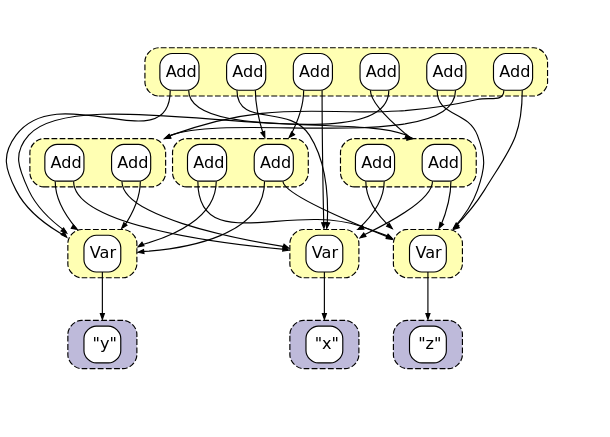
\includegraphics[width=\columnwidth]{addxyz}
    \caption{E-graph of the term $x + (y + z)$ after rewriting to saturation.}
    \label{egxyz}
\end{figure}

If we enter the term $x + ((y + z) + w)$ into the demo (Figure \ref{egxzw}), the resulting E-graph
is not even saturated, but the size has increased to the point where we reach the demo's built-in limit.

\begin{figure}[!ht] % suggests placing the figure here
    \centering % Centers the figure in the column
    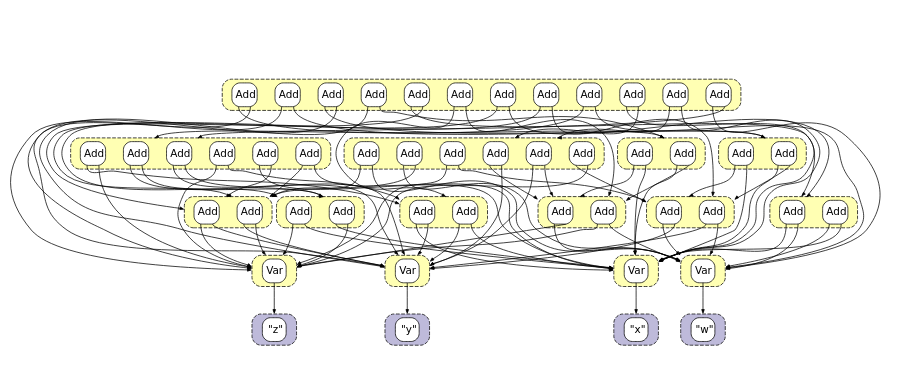
\includegraphics[width=\columnwidth]{add}
    \caption{E-graph of the term $x + ((y + z) + w)$ after a number of rewriting steps.}
    \label{egxzw}
\end{figure}

This graph shows that typically there are many syntactically-distinct terms that are equal modulo associativity and commutativity, which makes each equivalence class big, but also that there are many inequivalent \textit{subterms} that are referenced by the equivalence class of the input term.

The \textsc{Egg} library handles the application of identities with a backoff method, where
equations to apply are selected based on their weight, and the weight of an equation decreases when it fires. Any equation that suffers from blowup, like associativity or commutativity, will be fired less and less, in the hopes of finding more `interesting' equalities without having to run to saturation. This method isn't able to properly distinguish between `interesting' and `uninteresting' cases of associativity and commutativity, and it's also of no use when running to saturation.

In the rest of the paper, we will use `A/C' to refer to associativity and/or commutativity; namely, each of the three theories `A', `C', and `AC'. The theories are related, but each is independently useful.

To give an example of a theory with both A/C and `interesting' equalities, we extend the theory from above (containing only the function Add and the AC equations) with a function $f$, with the theory now containing $\forall ab. f(a + b) + 1 = f(a) + f(b)$ in addition to the AC identities from before. We also allow integer constants, and add all arithmetic identities to our theory, e.g. $1+1=2$. We begin with the term $f(x) + (f(y) + f(z))$. We would like to discover that this input term is equal to $f(x + (y + z)) + 2$, using the reasoning

\begin{align*}
	&f(x) + (f(y) + f(z)) = \\
	&f(x) + (f(y + z) + 1) = \\
	&(f(x) + f(y + z)) + 1 = \\
	&(f(x + (y + z)) + 1) + 1 = \\
	&f(x + (y + z)) + (1 + 1) = \\
	&f(x + (y + z)) + 2
\end{align*}

As we can see in Figure \ref{egf1}, the E-graph is on the way to discovering this, having for instance generated an equivalence class for the constant $2$, but hits the demo's limit again before completing this proof. While this example may be a toy example on a rather limited demo, it shows the extent to which A/C can clutter up the E-graph with many nodes that are not essential to a desired proof. Our equational proof above only needs to use associativity twice.

\begin{figure}[!ht] % suggests placing the figure here
    \centering % Centers the figure in the column
    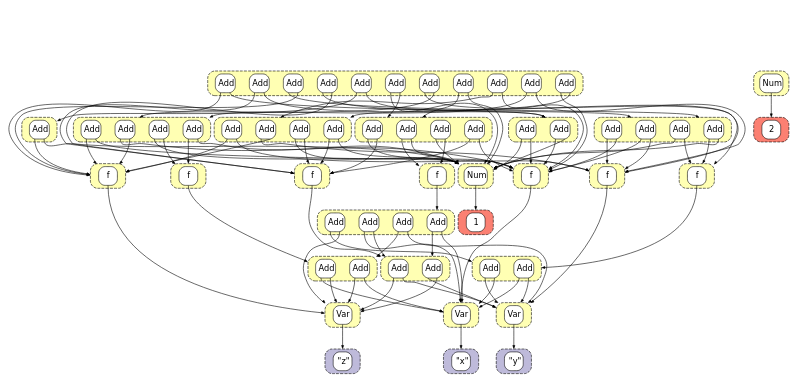
\includegraphics[width=\columnwidth]{addf1xyz}
    \caption{E-graph of the term $f(x) + (f(y) + f(z))$ after a number of rewriting steps.}
    \label{egf1}
\end{figure}

One could attempt to deal with AC ahead-of-time by automatically generating derived equations with a na\"ive `completion-like' method, e.g. deriving $f(a+b) + (1 + c) = (f(a) + f(b)) + c$ and $1 + f(a+b) = f(a) + f(b)$ from the source equation. This method is not in general complete: in the AC case, we would need infinitely many equations to handle matching at an arbitrary distance, as we can see with the term
$f(x+y) + (z_1 + (z_2 + \ldots (z_n + 1) \ldots))$. Here, any pattern that can determine that both $f(x+y)$ and $1$ are subterms, and therefore that there is a match modulo AC, must have $n$ auxiliary variables to capture (and ignore) each $z_n$ that stand between the $f(x+y)$ and the $1$.

This gives some idea of the difficulty in simply preprocessing the input theory and set of terms, and motivates considering a modification to the E-graph representation and algorithms themselves.

\subsection{Prior work on reasoning modulo theories}
There have been various proposals to alter the E-graph algorithms to, at least partially, solve the exponential size problem for A/C and similarly problematic theories. We focus on the paper at \textsc{Egraphs} 2025 by Zucker \cite{zucker2025omelets}, which introduces the notion of E-graphs Modulo Theories. The name is inspired by \emph{Satisfiability Modulo Theories} (SMT) solvers, which have seen significant improvements in speed and capabilities in recent decades. SMT solvers don't precisely solve
the same problems as E-graphs, but there is significant overlap in that they are both methods of theorem-proving in fragments of first-order logic. Modern SMT solvers use knowledge of a variety of built-in theories to solve input problems quickly.

The idea of E-graphs Modulo Theories is to take inspiration from SMT solvers and extend the E-graph mechanism with specific built-in theories. For example, as demonstrated above, the generic mechanisms of E-graphs handle A/C poorly, but there are methods to efficiently reason about terms modulo these identities.

\subsection{EMTs: an intuitive picture}
The key differences between EMTs and standard E-graphs is that we now represent our graph \emph{modulo theories}, so that, say, a single node that in a standard E-graph would represent $x+(y+z)$ is now taken to represent the 12 equivalent re-ordered and re-associated terms modulo AC. In order to achieve this, we need two key ingredients: when adding nodes to a graph, we need to \emph{canonicalize} them to one of the equivalent terms, so that, say, if we add $x+y$ and $y+x$ they will be canonicalized to the same representing term and thus considered to be identical. Canonizers for a variety of theories are well-known, and mostly involve making particular choices, such as imposing an ordering on terms and choosing that association will canonically be to the right. The harder problem is \emph{matching modulo theories}.

As an example of matching modulo theories, consider the equation we introduced above: $f(a + b) + 1 = f(a) + f(b)$. If we consider AC to be a built-in theory, then, when we match this against the term
$f(x+y) + (1 + f(z))$, we need a way to automatically determine that this term is equivalent to $(f(x+y) + 1) + f(z)$, and so contains a subterm that matches the pattern; thus the original term can be rewritten to $(f(x) + f(y)) + f(z)$. Besides AC, we might, for instance, also consider matching modulo the laws of negation, so that $f(x+y)$ itself can be matched to the left-hand side, and rewritten to $(f(x) + f(y)) - 1$.

First, we introduce our term $f(x) + (f(y) + f(z))$ (Figure \ref{egmt1}).

\begin{figure}[!ht] % suggests placing the figure here
    \centering % Centers the figure in the column
    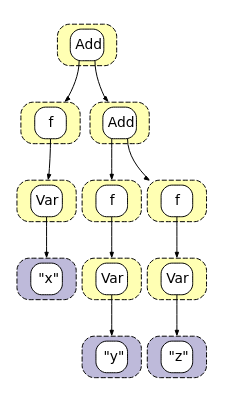
\includegraphics[width=0.3\columnwidth]{addmt1}
    \caption{E-graph of the term $f(x) + (f(y) + f(z))$ modulo AC}
    \label{egmt1}
\end{figure}

This term is canonized by an AC canonizer that right-associates terms and orders variables according to $x < y < z$. The canonization step ensures that each commutation or association of a term that is added only exists in the graph in a single form.

Next, we match and apply three instances of the identity $f(a + b) + 1 = f(a) + f(b)$. Since we are working modulo AC, instead of waiting for A or C rewrite rules to fire in order to `expose' the relevant match, we will instead to find matches of $f(a) + f(b)$ \emph{up to AC}.

An efficient algorithm for this matching will be given later, but note that the problem is decidable since there are only finitely many e-classes in the graph, and thus we could na\"ively enumerate all terms of the form $f(x) + f(y)$ where $f(x)$ and $f(y)$ are in the graph.

Adding the substituted instances of the left-hand side of the identity to the graph, we get the following E-graph with 10 new e-classes (Figure \ref{egmt2})

\begin{figure}[!ht] % suggests placing the figure here
    \centering % Centers the figure in the column
    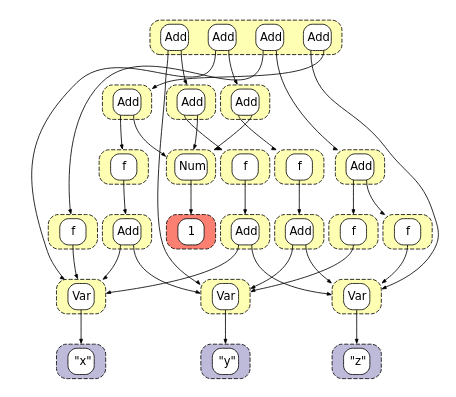
\includegraphics[width=0.8\columnwidth]{addmt2}
    \caption{E-graph of the term $f(x) + (f(y) + f(z))$ modulo AC after 1 rewriting step}
    \label{egmt2}
\end{figure}

We apply three more instances of the same identity, but these all generate the same new terms, so nothing changes (Figure \ref{egmt3}).

\begin{figure}[!ht] % suggests placing the figure here
    \centering % Centers the figure in the column
    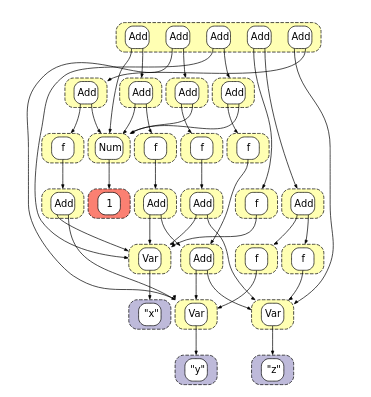
\includegraphics[width=0.8\columnwidth]{addmt3}
    \caption{E-graph of the term $f(x) + (f(y) + f(z))$ modulo AC after 2 rewriting steps}
    \label{egmt3}
\end{figure}

Finally, we use $1+1=2$ and reach saturation (Figure \ref{egmt4}).

\begin{figure}[!ht] % suggests placing the figure here
    \centering % Centers the figure in the column
    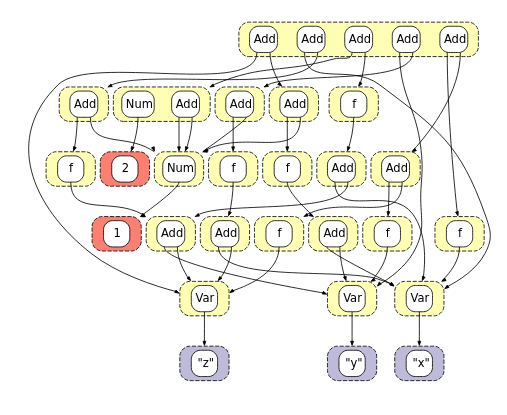
\includegraphics[width=0.8\columnwidth]{addmt4}
    \caption{E-graph of the term $f(x) + (f(y) + f(z))$ modulo AC after 3 rewriting steps, reaching saturation}
    \label{egmt4}
\end{figure}

We see that by working modulo AC, we reach saturation with only a few extra equivalence classes added, and no extra nodes to represent all the ways to commute and re-associate any uses of Add. Like with standard E-graphs, we are able to quickly discover the desired equality without any form of goal-directed search; we just need to run to saturation to discover all possible equalities from our input. The main technical challenge will be an efficient algorithm for matching modulo theories.

\subsubsection{Zucker's algorithm}
Zucker \citep{zucker2025omelets} provides a sketch of an \textit{incomplete} an algorithm to do matching. The procedure is as follows: enumerate all instances of the pattern with variables substituted for existing E-classes, and pass them all through the canonizer. Then, for the set of canonized results, check if it is in the graph, and if so, we have found a match.

Zucker's algorithm works for the example above, but it is not \textit{complete}. A counterexample to completeness is the following: consider the term $x + (y + z)$ and the pattern $a + b$. We would like to produce the match $\{a \mapsto x + y, b \mapsto z\}$, but the term $x + y$ is not a subterm of the original. If we consider the term $x + (-x + y)$ modulo A, with the rewrite rule $x + -x = 0$, then the LHS of the rule $x + -x$ will never match the term, despite the fact it is an `implied' subterm (modulo A) of the term the graph represents. Thus, matching with Zucker's algorithm will never discover the equation $x + (-x + y) = 0 + y$.

\subsection{Structured E-ids and matching modulo theories}
(TODO: this section lacks both technical elegance and helpful pictures)

In standard E-graphs we work over a set of equivalence classes with atomic \textbf{E-id}s, which we represent schematically as $e_i$. To move to EMTs, we will instead work with \textbf{structured E-id}s (SEID) which are canonical terms in the theory with atomic E-ids as variables. For instance, for E-ids $e_1, e_2$, and working with an associative binary operator $+$, $e_1 + e_2$ and $e_1 + (e_2 + e_1)$ will be structured E-ids, assuming we canonize by right association, while $(e_1 + e_2) + e_2$ will not be considered a structured E-id.

The key step in formalizing the matching problem is to establish a correspondence between EMTs and E-graphs such that the corresponding E-graph for an EMT explicitly represents all nodes that are equivalent under the theory to the `canonical' representative in the EMT.

To simplify, we will dispense with the explicit representation of the operation handled by the theory in the graph (as usual, we call it $+$ in the following discussion). Instead, we will introduce an auxiliary table of \textit{known structured E-ids}.

So, to represent $x + y + x$ with an A operator $+$, we will have an E-graph with two distinct e-classes for $x$ and $y$, and no other function symbols. Instead, in a side table, we will list $x + (y + x)$ as a known SEID.

Each known SEID behaves like ordinary E-ids in that it can have parent edges and similar metadata. For instance, with the term $f(x + y)$, the SEID $e_1 + e_2$ representing $x + y$ will have a pointer to the function node $f$. Equivalently, we have a graph that doesn't just contain term fragments over E-ids (e.g. $g(e_3)$, but term fragments over SEIDs (e.g. $f(e_1 + e_2)$).

Define an \textbf{implied subterm} of an EMT as follows:
\begin{itemize}
	\item for A, if $e_1 + \ldots (e_i + \ldots (e_j + \ldots)$ is a known SEID, then $e_i + (\ldots e_j)$ is an implied subterm. Equivalently, if we treat the canonical form of SEIDs as a list, then the implied subterm relation is just the sublist (substring) relation.
	\item for C, if a binary tree of $+$s and atomic E-ids is a known SEID, then any subtree of that tree, possibly with branches swapped, is an implied subterm.
	\item for AC, if a $e_1 + (\ldots e_n)$ is a known SEID, then any tree of elements of the $e_i$s, where the multiplicity of each $e_i$ in the tree is less than the number of occurences in the SEID, is an implied subterm. To illustrate the multiplicity requirement: if $e_1 + (e_2 + e_1)$ is an SEID, then $(e_1 + e_1) + e_2$ is an implied subterm while $e_1 + (e_ 2 + e_2)$ isn't.
\end{itemize}

The \textbf{implied expanded E-graph} is the E-graph corresponding to an EMT such that all implied subterms are expressed as explicit E-graph nodes.

Then, a complete matcher for an EMT is one that returns all assignments of (not necessarily known) SEIDs to pattern variables such that all matches in the implied expanded e-graph are covered by an SEID.

\subsection{Algorithms for matching and joins}
\textsc{Egg} uses the Rete algorithm \cite{forgy1989rete}, an incremental algorithm for standard E-matching.

It is pointed out by Zhang et al. in \citep{zhang2021relational} that E-graph matching is simply a \textit{conjunctive query} over the term graph viewed as a relation, which can be solved by algorithms used in databases for computing joins. The recent work on
Worst-Case Optimal Join (WCOJ) algorithms \cite{ngo2018worst} provides algorithms that are asymptotically better join performance than traditional binary joins, and there is also work on Free Joins \cite{wang2023free}, which provide a spectrum of algorithms that trade off between the asymptotic optimally of WCOJs with the practical speed advantages of binary joins. Zhang et al. explore the application of WCOJ algorithms to E-graph matching, showing significant performance improvements over Rete's algorithm, while not making any use of incrementality at all.

\section{Aims and timeline}
\subsection{Theoretical developments}
\subsubsection{Improving the description of the matching problem}
The above description is rather inelegant. A more clear and detailed description is needed.

Target date: Monday, week 6 (2nd of February)

\subsubsection{Diagrammatic free joins}
The various algorithms for matching discussed fit into a framework of *join plans* \cite{wang2023free} where they can be expressed as rearrangements of the same underlying conjunctive query. To be more specific, conjunctive queries fit directly into the diagrammatic language of string diagrams over monoidal categories \citep{selinger2010survey}, which I aim to use as a clarifying way to formulate the different `directions' of matching and the asymptotic tradeoffs. This is an extension and formalization of the syntax for various join plans given in the paper on Free Joins \cite{wang2023free}.

This formulation is clarifying but not trivial, in the sense that there are different performance costs to the various ways of expressing a conjunctive query despite them being algebraically equivalent.

I aim to write up a description of this diagrammatic formulation.

Note that the `modulo theories' part of matching cannot be described simply as a rearrangement of diagrams; there is a little bit extra needed.

Target date: Monday, week 7 (9th of February)

\subsubsection{Literature review of theory combination, and a logical description of structured E-ids}
There is an existing literature on reasoning with the combination of multiple theories, e.g. Shostak's algorithm \cite{raniseringeissentran2005congclos}. I aim to have reviewed enough literature to get a good idea how any E-graph based approach compares.

Also, I have derived a reasonably simple way to formalize Zucker's notion of `structured E-id', also described above. It would be nice to phrase this in terms of existing literature on theory combinations.

Target date: Tuesday, week 8 (17th of February)

\subsection{Describe how existing matching approaches fit into the join-diagram view}
An extension of the join-diagram work.

Target date: Tuesday, week 9 (24th of February)

\subsection{Describe the matching algorithm modulo one of A or C in terms of join diagrams}
Of course, we will also describe it more abstractly in a way independent of the join-plan. Still, the join-diagram approach is nice in general to describe complicated relational manipulations.

Target date: Monday, week 11 (9th of March)

\subsection{Implementation}
\subsection{Implement the infrastructure of the E-graph library: joins, join plans, the E-graph structure, and a saturation loop}
Target date: Monday, week 15 (6th of April)

\subsection{Implement the modulo-theory algorithm into the library}
Target date: Monday, week 16 (13th of April)

\subsection{Benchmarking}
\subsection{Collect a benchmark suite of problems}
I will need to decide if time-to-saturation is a good metric, as many existing cases don't run to saturation, and in many cases this is provably impossible. It is likely we will need to use the somewhat less precise metric of time to prove a particular desired `target' equation, which is more dependent on ordering of phases and so forth.

Target date: Wednesday, week 17 (22nd of April)

\subsection{Run benchmarks}
We want to try both various join plans and with/without the modulo-theories aspect. It will be important to see to what extent the various join plans make a difference, and also to test out the effectiveness of Zucker's incomplete matcher.

Target date: Wednesday, week 18 (29th of April)

\subsection{Finishing the report and giving the presentation}
Remainder of time in May

\section{Draft thesis structure}
\begin{enumerate}
	\item Introduction: a conceptual overview, few technical details
	\item Part 1: Background
		\begin{enumerate}
			\item Algebraic notions (signatures, terms, theories, definition of A/C)
			\item Relation notions (relations, conjunctive queries, flattening of patterns, matching, joins)
			\item E-graphs
				\begin{enumerate}
					\item Union-find and transitive closure
					\item Congruence closure
					\item Rewriting and saturation
					\item E-graphs under A/C
					\item Existing approaches to handle A/C (backoff, completion-type methods)
					\item Note on completeness (or potential lack thereof)
				\end{enumerate}
			\item A/C (how to canonize, etc.)
			\item Prior work on theory composition (including E-graphs and EMTs as theory composition)
		\end{enumerate}
	\item Part 2: Join plans
		\begin{enumerate}
			\item Diagrams of relations (mentioning the Free Join paper)
			\item Sequentializing diagrams
			\item The input/output distinction and indexing
			\item Estimating the cost of a plan
			\item Binary joins
			\item Worst-case optimal joins
			\item Top-down and bottom-up
			\item Representing E-graphs
			\item Theory nodes in join plans
			\item Incrementalizing joins \& Rete's algorithm
		\end{enumerate}
	\item Part 3: EMT(A/C) description in detail
		\begin{enumerate}
			\item EMTs and structured E-ids
			\item Implied subterms (including Equality of implied subterm)
			\item The matching specification
			\item Concrete matcher for A
			\item Concrete matcher for C
			\item Concrete matcher for A/C
		\end{enumerate}
	\item Part 4: Implementation
		\begin{enumerate}
			\item Implementing joins
			\item Implementing matching
			\item The outer loop
			\item Various strategies for the outer loop
			\item The benchmark cases
			\item Results
			\item Discussion
		\end{enumerate}
	\item Conclusion
\end{enumerate}

\section{Limitations}
\subsection{Detailed microbenchmarking}
I am hoping that algorithmic improvements will be sufficient to cause noticeable differences in the benchmark scores without worrying too much about the details of the micro-optimizations that might be applicable.

\subsection{Incompleteness}
E-graphs are already not complete for reasoning in some cases. It would be nice to prove that EMTs are `at least as complete' as E-graphs, but my intuitions and knowledge around completeness is not strong enough that I can be sure that I can do such a proof.

\subsection{Is matching possible?}
I initially believed that Zucker's algorithm, which is much simpler than the algorithm described in my proposal, was complete. However, this is not the case (see above). Still, the problem is at least decidable for A/C (proof given above, but fundamentally this rests on finiteness). So, while I cannot guarantee that the EMT approach will be much better than the standard one, I am confident that there is \textit{some} form of EMT that can be implemented and benchmarked, even if na\"ive.

Still, there is scope to reduce the problem if this turns out to be more difficult than expected: even Zucker's incomplete matcher might be useful in practice as a fast matcher to be run several times in between a slower, complete matcher, or we could use a `seeding' method to add extra E-nodes that Zucker's matcher would miss, due to them not being directly present in the E-graph. Thus, there is always space for exploration and practical benchmarking here despite the possibility of theoretical hurdles.

\section{Summary}
We propose to develop a family of algorithms for matching in an E-graph modulo A, C, and AC, where the exact algorithm depends on a given join plan, a formal notion to be introduced that includes the existing notions of top-down and bottom-up matching.

\section{References}

\printbibliography

\end{document}